%%%%%%%%%%%%%%%%%%%%%%%%%%%%%%%%%%%%%%%%%%%%%%%%%%%%%%%%%%%%%%%%%%
%%%%%%%% ICML 2014 EXAMPLE LATEX SUBMISSION FILE %%%%%%%%%%%%%%%%%
%%%%%%%%%%%%%%%%%%%%%%%%%%%%%%%%%%%%%%%%%%%%%%%%%%%%%%%%%%%%%%%%%%

% Use the following line _only_ if you're still using LaTeX 2.09.
%\documentstyle[icml2014,epsf,natbib]{article}
% If you rely on Latex2e packages, like most moden people use this:
\documentclass{article}


% use Times
\usepackage{times}
\usepackage{geometry,amsmath}

% For figures
\usepackage{graphicx} % more modern
%\usepackage{epsfig} % less modern
\usepackage{subfigure} 


% For citations
\usepackage{natbib}
\usepackage{url}

% For algorithms
\usepackage{algorithm}
\usepackage{algorithmic}

% As of 2011, we use the hyperref package to produce hyperlinks in the
% resulting PDF.  If this breaks your system, please commend out the
% following usepackage line and replace \usepackage{icml2014} with
% \usepackage[nohyperref]{icml2014} above.
%\usepackage{hyperref}

% Packages hyperref and algorithmic misbehave sometimes.  We can fix
% this with the following command.
\newcommand{\theHalgorithm}{\arabic{algorithm}}

% Employ the following version of the ``usepackage'' statement for
% submitting the draft version of the paper for review.  This will set
% the note in the first column to ``Under review.  Do not distribute.''
\usepackage{icml2014}


% The \icmltitle you define below is probably too long as a header.
% Therefore, a short form for the running title is supplied here:
\icmltitlerunning{de Villalobos, Lautman, Yim}

%%%%%%%%%% Start TeXmacs macros
\newcommand{\nosymbol}{}
\newcommand{\tmop}[1]{\ensuremath{\operatorname{#1}}}
%%%%%%%%%% End TeXmacs macros

\begin{document} 

\twocolumn[
\icmltitle{Penn Project Report\\Machine Learning in Real Time Character Recognition}

% It is OKAY to include author information, even for blind
% submissions: the style file will automatically remove it for you
% unless you've provided the [accepted] option to the icml2014
% package.
\icmlauthor{Francisco de Villalobos}{frade@seas.upenn.edu}
\icmlauthor{Michael Lautman}{mlautman@seas.upenn.edu}
\icmlauthor{Justin Yim}{yimj@seas.upenn.edu}

% You may provide any keywords that you 
% find helpful for describing your paper; these are used to populate 
% the "keywords" metadata in the PDF but will not be shown in the document
\icmlkeywords{machine learning, character recognition, kaman filter}


\vskip 0.3in
]

\begin{abstract} 
This paper presents a MEMS based digital pen for handwriting recognition. While there are several devices which are capable of digitizing handwritten notes, all commercially available devices require secondary hardware to function. We propose a single device solution for digitizing text as it is written on a page. By calculating the dynamics of the pen from IMU measurements, we are able to estimate the pen tip accelerations and rotations as a function of time. We evaluated SVCs, decision trees, Ada-Boost, and logistic regression learning algorithms based on their ability to recognize handwritten characters and achieved 96.2 \% accuracy using an SVC with a lineal kernel.
\end{abstract} 

\section{Prototype}
In this section we give a brief summary of the hardware incorporated into the proposed device. We first describe the mechanical device before then discussing the electronics. 

\subsection{Hardware}
The pen layout and body was designed in CAD (pictured below) to ensure appropriate packing of components. The clear body was 3D printed in ABS in the University's prototyping labs. 

\begin{figure}[H]
	\centering
	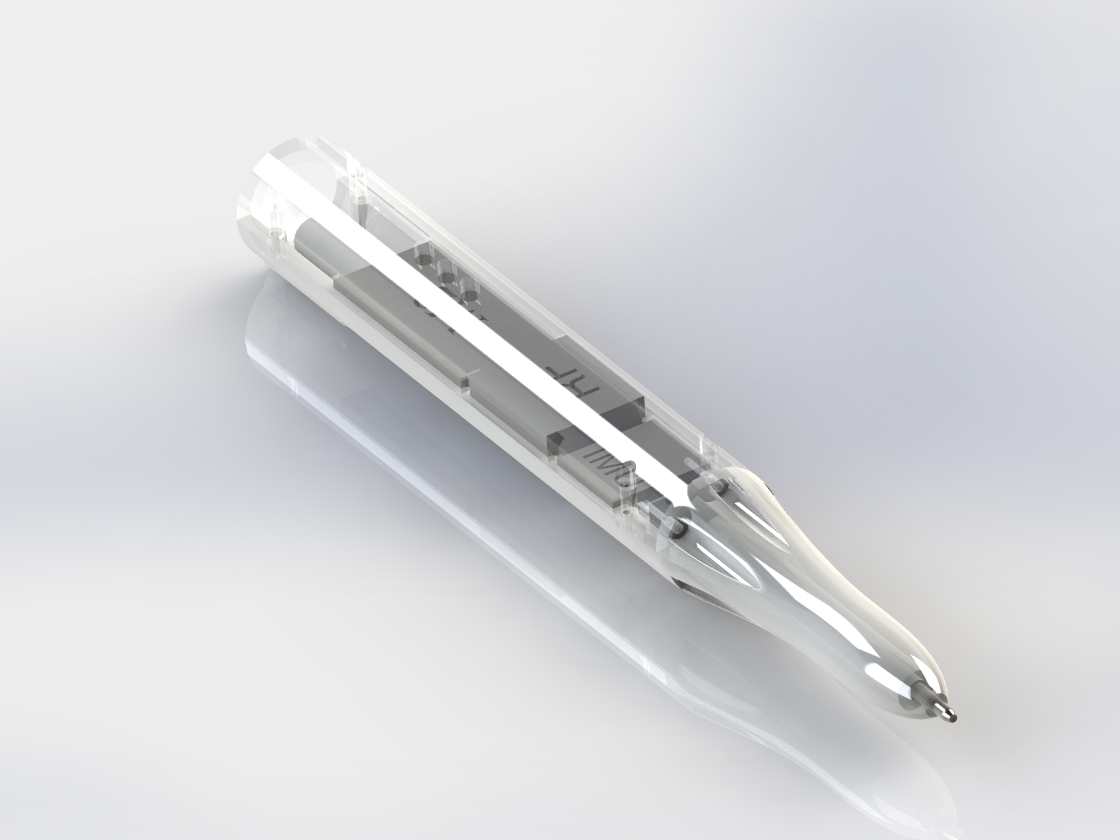
\includegraphics[width=0.5\textwidth, height= 5cm]{pen_render.png}
	\caption{Rendering of the 3D printed model of the penn}
\end{figure}

\subsection{Electronics}
An ATMega32u4 microcontroller provides on-board processing and interfaces to the wireless module, IMU, switch, and indicator LEDs. Two Nordic nRF24LE1 transceivers handle wireless communication between the pen and base station computer. Inertial measurements are provided by an MPU6050 digital IMU with configurable gain triaxial accelerometers and gyroscopes. A Honeywell HMC5883L triaxial magnetometer provides a reference to earth's magnetic field for orientation. A switch behind the pen tip detects contact with the page for character segmentation. Three LEDs on the case display pen state. The pen also includes on-board batteries, power management, and an on-off switch to track idle and writing time of the pen, which translates in useful and un-useful data.

\subsection{Filtering the data}

The raw data from the IMU pose issues for learning algorithms. Sources of variance can include posture, handed-ness, roll angle of the pen, and sensor drift. To minimize sources of error, we compute the trajectory of the pen tip on the page to generate features in a four step process. 
\begin{enumerate}
  \item IMU measurements are scaled to engineering units and are low-pass filtered to remove high frequency noise from vibration.
  \item We use Madgwick's open source Kalman filter and attitude estimator to find the orientation of the pen relative to the page.
  \item We transform the IMU measurements into the ground frame relative to the page and double-integrate the acceleration to estimate the displacements of the pen tip.
  \item Finally, the position and velocity estimates are high-pass filtered to remove drift.
\end{enumerate}

From this IMU data processing we obtain the x,y,z position, velocity, and acceleration of the pen in the page frame as well as the euler angles and angular rates of the pen in the page frame at 300Hz sample rate. \newline
Down below we can see how the user interface for testing looks like, and an example of the trajectory reconstruction of a "g" letter. In the MATLAB plots we can see all the readings of the IMU in real time, the attitude estimation of the penn in 3D (Which corresponds to the real position of the penn with a very slight delay), and the real time trajectory reconstruction of the writings with other parameters.

\begin{figure}[H]
\centering
    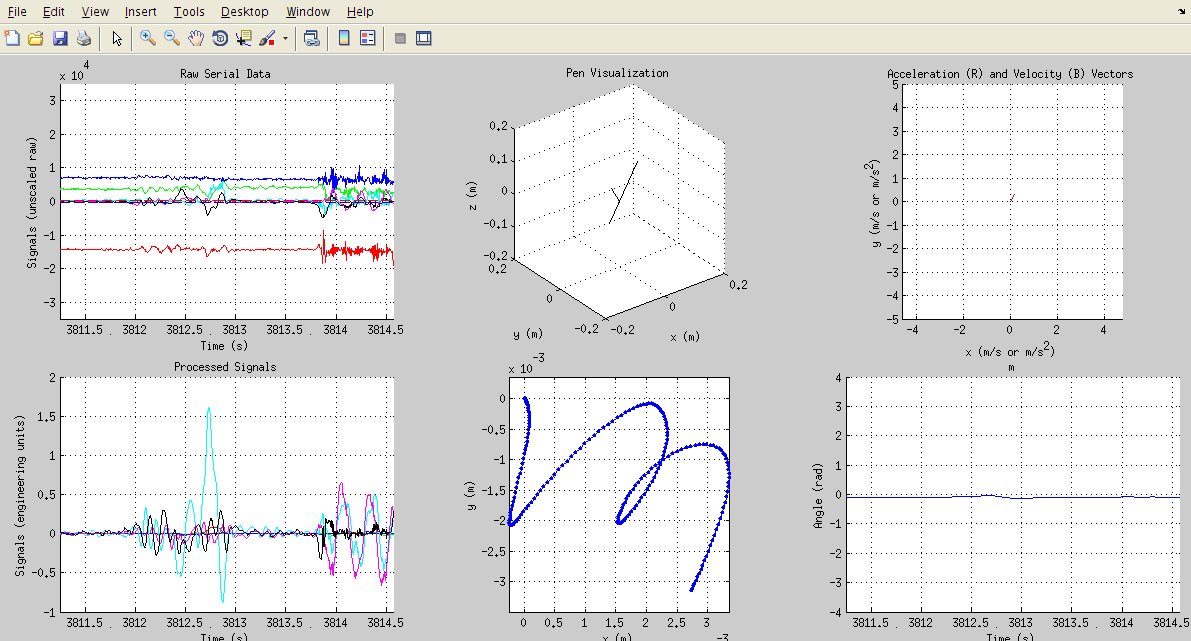
\includegraphics[width=0.5\textwidth, height= 5cm]{interface.png}
    \caption{Writing interface for character recognition}
\end{figure}

\begin{figure}[H]
\centering
    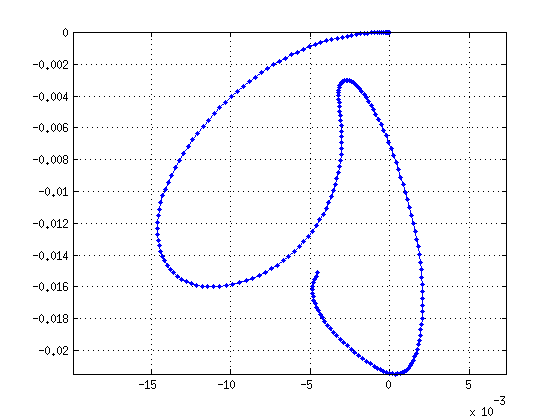
\includegraphics[width=0.5\textwidth, height= 5cm]{g.png}
    \caption{Recovered letter "g"}
\end{figure}

\subsection{Coordinate Transformation}
Accelerations and rotations of the pen body measured at the IMU are translated to the tip by the following transform:

\textbf{P}: location of the IMU \\
\textbf{O}: origin of frame G on the page \\
\textbf{frame G}: SRT fixed to the page with origin O (ground frame) \\
\textbf{frame M}: SRT fixed to the pen at the IMU with origin at point P (pen frame) \\
\textbf{Q}: location of the pen tip \\
$\underset{\mbox{\textasciitilde}}{\tmop{\textbf{PQ}}}$: vector from the IMU origin to
the pen tip

The acceleration of the pen tip in the ground frame is given by:
\begin{align*}
  ^G \underset{\mbox{\textasciitilde}}{a}^Q =^G
  \underset{\mbox{\textasciitilde}}{a}^P +^M
  \underset{\mbox{\textasciitilde}}{a}^Q &+^G
  \underset{\mbox{\textasciitilde}}{\alpha}^P \times
  \underset{\mbox{\textasciitilde}}{\tmop{PQ}} + 2^G
  \underset{\mbox{\textasciitilde}}{w}^M \times^M
  \underset{\mbox{\textasciitilde}}{v}^Q + ... \\ &+ ^G 
  \underset{\mbox{\textasciitilde}}{w}^M \times \left(^G
  \underset{\mbox{\textasciitilde}}{w}^M \times
  \underset{\mbox{\textasciitilde}}{\tmop{PQ}} \right)
\end{align*}
Since point Q (the pen tip) is fixed in frame M (the pen frame), $^M
\underset{\mbox{\textasciitilde}}{a}^Q$ and $^M
\underset{\mbox{\textasciitilde}}{v}^Q$ are both 0. The above equation simplifies to:
\begin{eqnarray*}
  & ^G \underset{\mbox{\textasciitilde}}{a}^Q =^G
  \underset{\mbox{\textasciitilde}}{a}^P +^G
  \underset{\mbox{\textasciitilde}}{\alpha}^P \times
  \underset{\mbox{\textasciitilde}}{\tmop{PQ}} +^G
  \underset{\mbox{\textasciitilde}}{w}^M \times \left(^G
  \underset{\mbox{\textasciitilde}}{w}^M \times
  \underset{\mbox{\textasciitilde}}{\tmop{PQ}} \right) & 
\end{eqnarray*}
The IMU measures accelerations and angular velocities of frame M relative to frame G expressed in frame M. \ Using the attitude estimate, these measurements can be rotated into frame G to produce $^G
\underset{\mbox{\textasciitilde}}{a}^P$ and $^G
\underset{\mbox{\textasciitilde}}{w}^M \nosymbol$. \ The angular acceleration
$^G \underset{\mbox{\textasciitilde}}{\alpha}^P$ is obtained by numerically
differentiating $^G \underset{\mbox{\textasciitilde}}{w}^M$.

The trajectory of the pen tip in the page frame is obtained by twice-integrating $^G \underset{\mbox{\textasciitilde}}{a}^Q$.
Since the velocity and position are integrations of noisy signals they are prone to very significant drift over time. To counteract this drift, the position and velocity estimates are re-zeroed at the start of every character and both the velocity and position are high pass filtered. The resulting trajectory can be plotted in the plane to approximate the appearance of the character on the page. This trajectory image is sampled to produce a black and white image which is then scaled and blurred to produce the final learning features.

\newpage
\section{Learning}

\subsection{Features}
To generate our feature vector, we find the mean, standard deviation, and RMS of each of the signals x, y, z position, velocity, and acceleration and euler angles and angular rates, then interpolate each of the signals to a uniform length.  Our feature vector consists of the character writing time, these interpolated signals, and their mean, standard deviation, and RMS.  This generates a feature vector of length 15*N + 46 where N is the interpolated signal length.  After feature vector generation we standardize our features.  
 
\subsection{Learning Algorithms}
We first tested Support Vector Machines with different Kernels to compare the results we were getting from them. This ones were all runned with 5 folds.

\begin{center}
    \begin{tabular}{ | c | c | c | c | c | r |}
    \hline
    $\textbf{Algo.}$ & $\textbf{Kernel}$  & $\textbf{param}$ & $\textbf{Sig Len}$ & $\textbf{Time(s)}$ & $\textbf{Acc.}$ \\ \hline
    SVC & linear & - & 10 & 2.114 & 96 $\%$ \\ \hline
    SVC & poly & 2 & 10 & 2.07 & 91 $\%$ \\ \hline
    SVC & poly & 3 & 100 & 6.681 & 91 $\%$ \\ \hline
    SVC & gaussian & 5E-1 & 10 & 5.057 & 3 $\%$ \\ \hline
    SVC & gaussian & 5E-4 & 10 & 2.124 & 77 $\%$ \\ \hline
    SVC & gaussian & 5E-5 & 10 & 3.05 & 29 $\%$ \\ \hline
    SVC & gaussian & 5E-4 & 100 & 11.357 & 93 $\%$ \\ \hline
    SVC & gaussian & 5E-5 & 100 & 13.709 & 82 $\%$ \\ \hline
    SVC & gaussian & 5E-3 & 1000 & 309.19 & 3 $\%$ \\ \hline
    
    \end{tabular}
\end{center}

As we can clearly see, while the linear and polynomial kernel do a pretty good job to classify the characters, the gaussian is VERY prone to subtle variations in the parameters, which makes it a non robust method for character recognition. The gaussian kernel smoothes everything if you don't have the correct parameters, and that is why it's a non reliable method for this application in particular. We can see how the performance for the gaussian kernel goes from 3 to 77\% and then back down to 10\% depending on the choice of gamma. And then once again changing the signal length we get very different performances. \newline
On the other side, we can see that the accuracy obtained by the polynomial kernel is not even affected by the degree of the same and the variations are little while it runs very fast. Better then, we get the best performance with the linear kernel, were we don't have to worry about the gamma or the polynomial degree.

As expected, decision trees perform poorly on this dataset.  Decision trees in general have lower predictive power than the other methods applied here.  Furthermore, we expect the ideal decision function to be much smoother non axis-aligned than the axes-parallel hyper-rectangles of decision trees can produce.  This is because the integrated time series features are highly correlated with one another.  Despite the smoothing of AdaBoost, AdaBoosted decision trees still underperformed other methods for some settings, and got over 97\% accuracy for some other setting, but taking a lot of extra time that is essential for the quickness of writing and 3\% increase in performance does not justify the speed of AdaBoost at this settings.

% Other algorithms tables
\begin{center}
    \begin{tabular}{ | c | c | c | c | c | r |}
    \hline
    $\textbf{Algorithm}$ & $\textbf{param}$ & $\textbf{Acc.}$ \\ \hline
    DT & depth=100 & 67.82 $\%$ \\ \hline
    DT & depth=200 & 68.24 $\%$ \\ \hline
    Log Reg & L1 penalty & 89.20 $\%$ \\ \hline
    Log Reg & L2 penalty & 89.47 $\%$ \\ \hline
    AdaBoost & k=7 c=1 & 70.11$\%$ \\ \hline
    AdaBoost & k=5 c=3 & 92.99 $\%$ \\ \hline
    
    \end{tabular}
\end{center}
In this table we have k being the k-folds and c being cross validation splits. We also tuned the depth of the Decision Tree and the number of estimators and the learning rate for the algorithm. This could all tune the accuracy that we got from it, but also influenced a lot the time that the 

Logistic regression performs well achieving accuracy, precision, and recall of 89\% with both l1 and l2 norm distance metrics.  
 
Several letters are very similar in stroke trajectory.  All learning algorithms struggled with these sets of letters more than other sets of letters as the confusion matrices reveal.  Similar letter pairs include o and 0, p and b, 9 and q, y and x, h and n, 0 and 6, 5 and 6, 7 and 8, v and r, m and k, and a and u.  Some of these letter pairs look visually different from each other, but are composed of similar stroke patterns (for example a script k and an m share the same vertical beginning stroke, direction reversal, loop and second direction reversal).


\section{Performance}
\subsection{Tested Algorithms}
The algorithms that were tested were SVCs with different kernels, Decision Trees, Logistic Regression with L1 and L2 penalties, and AdaBoost decision Stumps. While all of the performed with a lot more than random success, there were differences between them.

\subsection{Final Performance}

 As we can well see, even though the logistic regression gets ~89\% accuracy, the ones that do better are the SVCs with linear kernel. SVCs with linear kernels present a robust machine learning algorithm that is not going to be changed completely if we add a new feature to the feature vector for example. They perform quickly, efficiently, and accurately making them the best algorithm for the task. We will next compare some of the results between the SVCs with linear kernels and the Decision trees that among the ones that perform poorly, still get over 60\% accuracy.


We can observe how the true positives in the SVCs go steeper and faster into the true positive area, making less mistakes in all instances.
% Precision & recall, ROC, etc.
\begin{figure}[H]
	\centering
	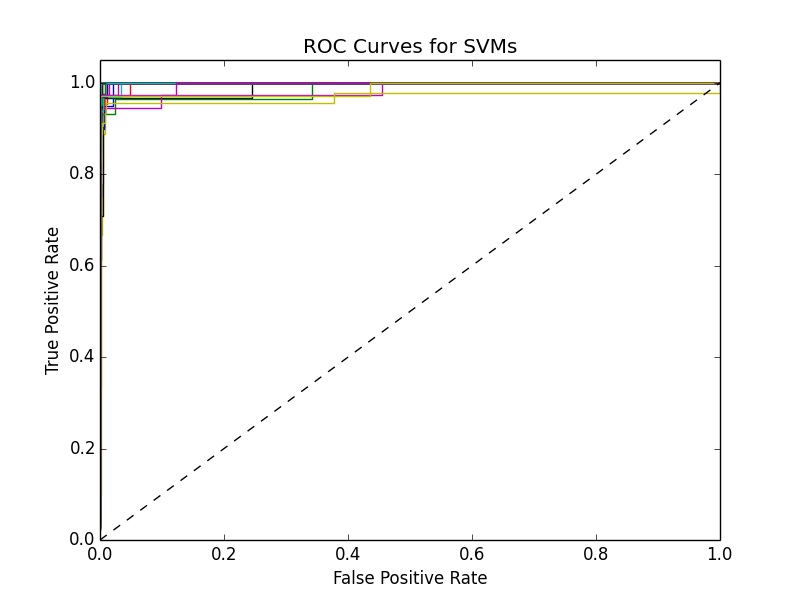
\includegraphics[width=0.5\textwidth, height= 5cm]{roc_svm_francisco__svm.png}
	\caption{ROC curves of an SVC with linear kernel}
\end{figure} 
\begin{figure}[H]
	\centering
	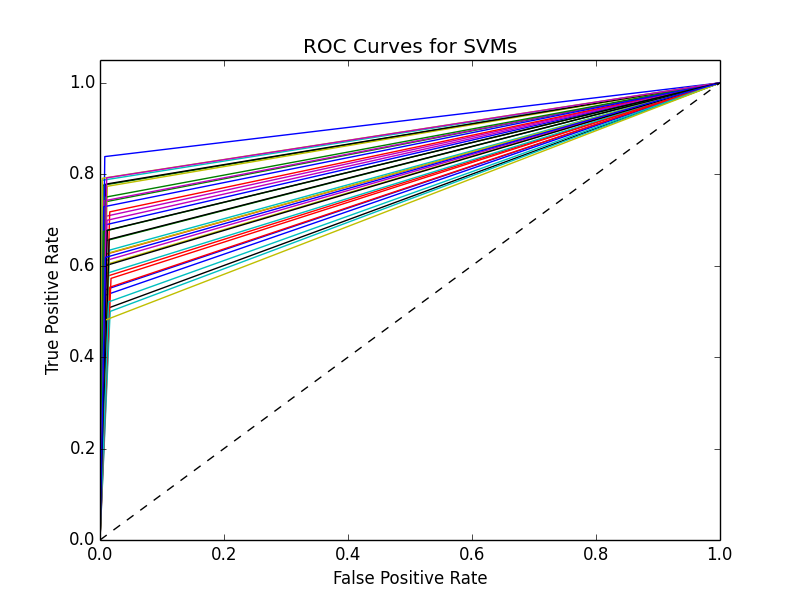
\includegraphics[width=0.5\textwidth, height= 5cm]{roc_tree1_dt.png}
	\caption{ROC curves of a Decision Tree with max depth = 100}
\end{figure} 
Next we will be looking at the confusion matrices of SVCs with linear kernel and Decision Trees. We will appreciate this index in the way that it visually and automatically compares the accuracy of a method to another, and which are the characters that are most commonly mis-classified.
% Confusion matrix
\begin{figure}[H]
	\centering
	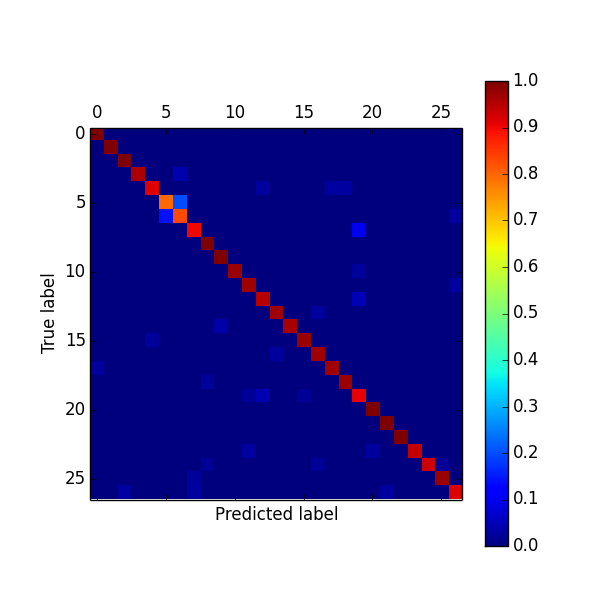
\includegraphics[width=0.5\textwidth, height= 5cm]{cm_svm_francisco__svm.png}
	\caption{Confusion Matrix of an SVC with linear kernel}
\end{figure} 
\begin{figure}[H]
	\centering
	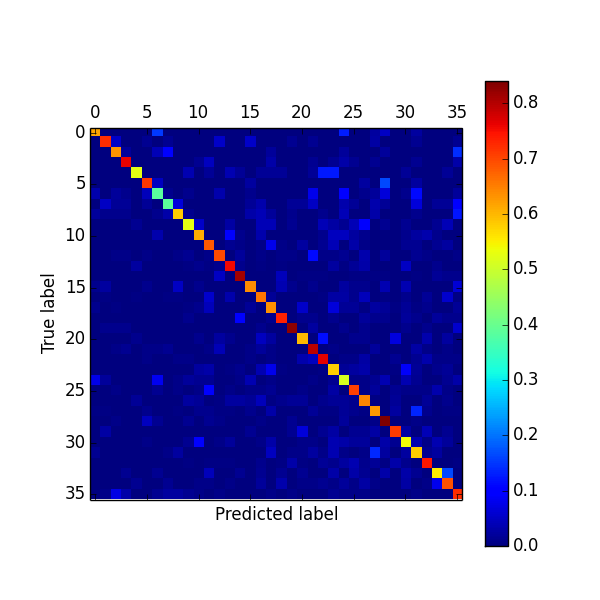
\includegraphics[width=0.5\textwidth, height= 5cm]{cm_tree1_dt.png}
	\caption{Conf. Matrix of a Decision Tree with max depth = 100}
\end{figure} 
We can observe in these confusion matrices how the diagonal is much stronger than the sides, meaning that most of the instances of a certain class are classified correctly, and that there are very little false positives and false negatives.
And it is visually clear how different the performance for these two methods is, because we can see a lot more light blue spots in the false positive area in decision trees for things that were mis-classified.


\section{Results}
Character recognition was achieved with a very high accuracy and implemented in real time in a real environment. The methods and equations listed above have proven successful and reliable.\newline
Here you can see a video of our interface, readings, character tracking, and an example of a "Hello World" recognition: 
\url{https://www.youtube.com/watch?v=L0AaqIswKBE&list=UUEdPimfOpE81_NbsL7sXQhA&spfreload=10} \newline \newline
While very satisfied with the results, this is far from being a commercial product. But being that we could get this working in such a short period of time, I believe that with a couple of months of exclusive work on this devise, we could get into market a penn that implements Hidden Markov Models (While on our research we found that this algorithm could lead to smaller percentage errors) and has a very low percentage error, while at the same time is capable of doing some more advanced things like spaces, or math. A penn that could put math into your digital notes would be a great product that we believe can have a great success in real market, competing at a much lower price with products that rely on cameras to get similar results (While at the same time I have not seen one that performs adequately in math environments).

\section*{Acknowledgments} 
 
Attitude estimation Kalman Filter and initial approximation provided by \textbf{open-source} code from Sebastian Madgwick (July 2012), based on his paper \textbf{Estimation of IMU and MARG orientation using a gradient descent algorithm}.\\\\
For trajectory reconstruction, consulted Jeen-Shing Wang, Yu-Liang Hsu, and Jiun-Nan Liu's paper entitled \textbf{An Inertial-Measurement-Unit-Based Pen With a Trajectory Reconstruction Algorithm and Its Applications}.
%\bibliography{example_paper}
%\bibliographystyle{icml2014}

\end{document} 


% This document was modified from the file originally made available by
% Pat Langley and Andrea Danyluk for ICML-2K. This version was
% created by Lise Getoor and Tobias Scheffer, it was slightly modified  
% from the 2010 version by Thorsten Joachims & Johannes Fuernkranz, 
% slightly modified from the 2009 version by Kiri Wagstaff and 
% Sam Roweis's 2008 version, which is slightly modified from 
% Prasad Tadepalli's 2007 version which is a lightly 
% changed version of the previous year's version by Andrew Moore, 
% which was in turn edited from those of Kristian Kersting and 
% Codrina Lauth. Alex Smola contributed to the algorithmic style files.  
